%%%%%% a 18-array affymetric data %%%%%%%%%%%%%%%%%%
\subsection{An affymetric experiment}
This is a 18-array affymetric experiment. 
It used 3 mouse strains, three individuals
out of each strain (so there are nine mice) and did two
affymetric arrays for each individual. The experimental
design is shown in figure \ref{fig:abf1}. I hand picked
500 genes out of it to make the calculation runs faster.

Note that the data visualization and transformation
functions in {\tt R/maanova} are not
applicable to one-dye data (at this time). Model fitting
and statistical testing functions will work.

% figure for abf1 experiment
\begin{figure}[htbp]
\centering
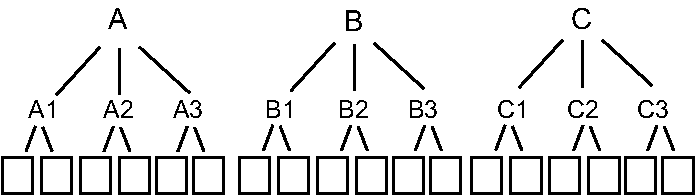
\includegraphics{abf1}
\caption{18-array affymetric experiment design}
\label{fig:abf1}
\end{figure}


% start code
\begin{enumerate}
\item Load in data \\
\begin{Sinput}
R> data(abf1)
\end{Sinput}

\item Make data object. There is no data transformation function
for affymetric array in {\tt R/maanova} at this time. So this
data set was pre-transformed using {\bf Affy} package in 
{\bf BioConductor}. So we should not take log transformation
in making data object.
\begin{Sinput}
R> abf1 <- createData(abf1.raw, 1, log.trans=F)
\end{Sinput}

\item Make model object and fit ANOVA model. We will treat 
the biological replicates as random effect.
Note that you cannot fit Array and Dye effect
for one-dye arrays.
\begin{Sinput}
R> model.full.mix <- makeModel(data=abf1, formula=~Strain+Sample, 
       random=~Sample)
R> anova.full.mix <- fitmaanova(abf1, model.full.mix)
\end{Sinput}

\item Do F-test on strain and generate volcano plot
\begin{Sinput}
R> test.Strain.mix <- matest(abf1, model.full.mix, term="Strain", 
          n.perm=100)
R> idx.mix <- volcano(test.Strain.mix)
\end{Sinput}

\end{enumerate}

